\section{Limit Setting}
\label{sec:limits}
We use the ``Higgs Combination'' package \cite{cite:combine} for
setting exclusion limits. This package is a
RooStats\cite{cite:roostats}-based statistical analysis toolset
recommended by the CMS Higgs PAG.

For model-specific results, we consider the Technicolor, Leptophobic
$\Zo^\prime$, and WH/ZH signal models described in
Section~\ref{sec:NewPhysics}. These are subjected to the same analysis
selections as data and MC background. We also consider a generic Gaussian
signal model positioned at $150~\gev$ with $\sigma=15~\gev$,
representing a delta function convolved by the detector jet energy
resolution. The integral normalization of this signal is set to 1~pb as follows:

\begin{equation*}
  \textrm{norm} =  1~\textrm{pb} \times (\epsilon\times\cal{A})_{\textrm{WH}} \times \int \cal{L} \textrm{dt}
\end{equation*}

where
\begin{eqnarray*}
  (\epsilon\times\cal{A})_{\textrm{WH}} &=& \textrm{efficiency $\times$ acceptance measured for WH} \\
     \int \cal{L} \textrm{dt} &=& 5.0~\textrm{fb}^{-1}
\end{eqnarray*}

The values used for $\epsilon\times\cal{A}$ are shown in Table~\ref{tab:signals}.

We therefore take as inputs the residual dijet invariant mass
distributions for each signal model, data, and total background that
survive after analysis cuts. All of these distributions are segregated by lepton flavor and jet content, which represent independent
channel inputs to the limit setter. For a ``cut-and-count'' limit, we
integrate these distributions over a narrow window around $150~\gev$
that represents 1-2 sigma of the detector energy resolution and feed the
total yields to the limit setter. For shape-based limits, we supply
these distributions over the full range ($60-300~\gev$) in the form of
histograms to the limit setter.

%% %The datacard inputs to the combination package for the nominal limit
%% %therefore include those systematics that were deemed to be
%% %non-negligible.  These include the shape-based matching up/down and
%% %scale up/down variations, as well as background normalization
%% %uncertainty (1.75\% for the 2-jet bin and 3.35\% for the 3-jet bin)
%% %and a 4.5\% uncertainty for luminosity (signal only). A sample datacard
%% %is shown in Fig.~\ref{fig:sampledatacard}.

%% %\begin{figure}[h!]
%% %\footnotesize
%% %\begin{verbatim}
%% %imax 2 number of bins
%% %jmax 1 number of processes minus 1
%% %kmax 4 number of nuisance parameters
%% %----------------------------------------------------------------------------------
%% %shapes *       bn2jet  mjj_bn2jet.root $PROCESS_bn2jet $PROCESS_bn2jet_$SYSTEMATIC
%% %shapes *       bn3jet  mjj_bn3jet.root $PROCESS_bn3jet $PROCESS_bn3jet_$SYSTEMATIC
%% %----------------------------------------------------------------------------------
%% %bin          bn2jet   bn3jet 
%% %observation  43746.0  16567.0
%% %----------------------------------------------------------------------------------
%% %bin                               bn2jet      bn2jet      bn3jet      bn3jet    
%% %process                           Signal      Bckgrdtot   Signal      Bckgrdtot 
%% %process                           0           1           0           1         
%% %rate                              105.0000    43746.8400  17.5000     16567.4300
%% %----------------------------------------------------------------------------------
%% %Bkgdnorm                lnN       -           1.0175      -           1.0335    
%% %lumi                    lnN       1.045       -           1.045       -         
%% %matching                shape     -           1.0         -           1.0       
%% %scale                   shape     -           1.0         -           1.0       
%% %\end{verbatim}
%% %\caption{\label{fig:sampledatacard}A sample data-card combining the
%% %2-jet and 3-jet bins, with all systematics considered.}
%% %\end{figure}

The limit setter is then set to utilize the ``asymptotic CL$_{s}$''
\cite{cite:asympcls1,cite:asympcls2} method. The resulting observed limit, as well as
the median expected limit and 1- and 2-sigma error bands, are plotted.
%%%%%%%%%%%%%%%%%%%%%%%%%%%%%%
\subsection{Limits from full \texorpdfstring{5.0 fb${}^{-1}$}{5.0/fb} data sample (Runs: 2010+2011A+2011B)}
In Fig.~\ref{fig:FigLimitsFullData}a we show observed and expected values of the
CL${}_{S}$ statistic for the generic Gaussian signal model described above
as a function of the cross section $\sigma = \mu \times$~1~pb~$\times$~the branching fraction
for $W\to\ell\nu$, where $\mu$ is
known as the signal strength.
Upper limits on cross section computed at the 95\% confidence level (C.L.)
for technicolor, leptophobic $\Zo^\prime$, and WH ($M_H = 150$~GeV) are 
shown in Fig.~\ref{fig:FigLimitsFullData}b.
We set a 95\% C.L. upper limit of 1.1 pb on the production cross section 
$\times BR(W\to\ell\nu)$ for such resonances.
%%%%%%%%%%%%%%%%%%%
\begin{figure}[bthp]
%%\subfigure[]{
%%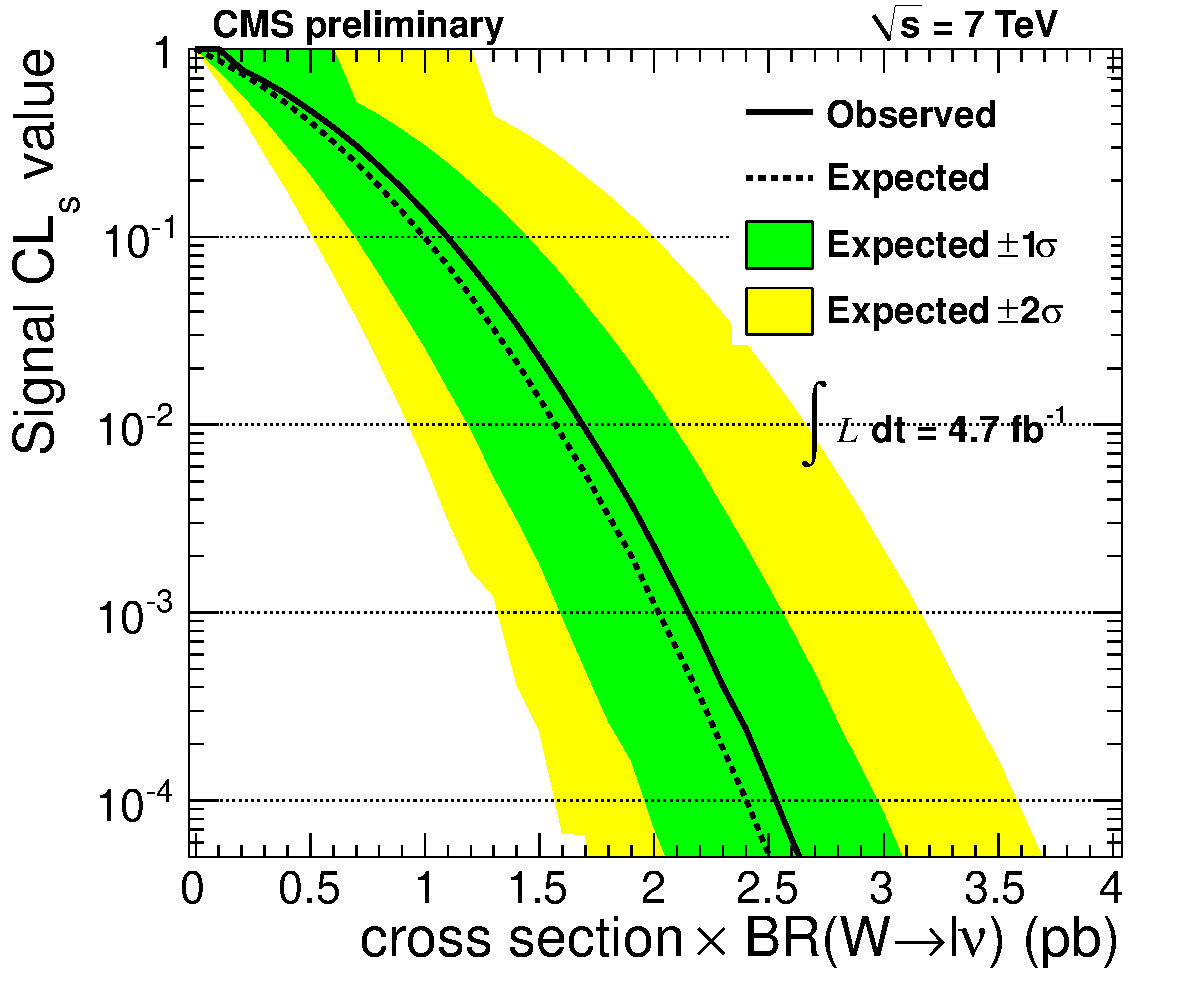
\includegraphics[width=0.45\textwidth]{figs/mjjpvalues_gs2+3jet_4p7fb.pdf}
%%}
%%\subfigure[]{
%%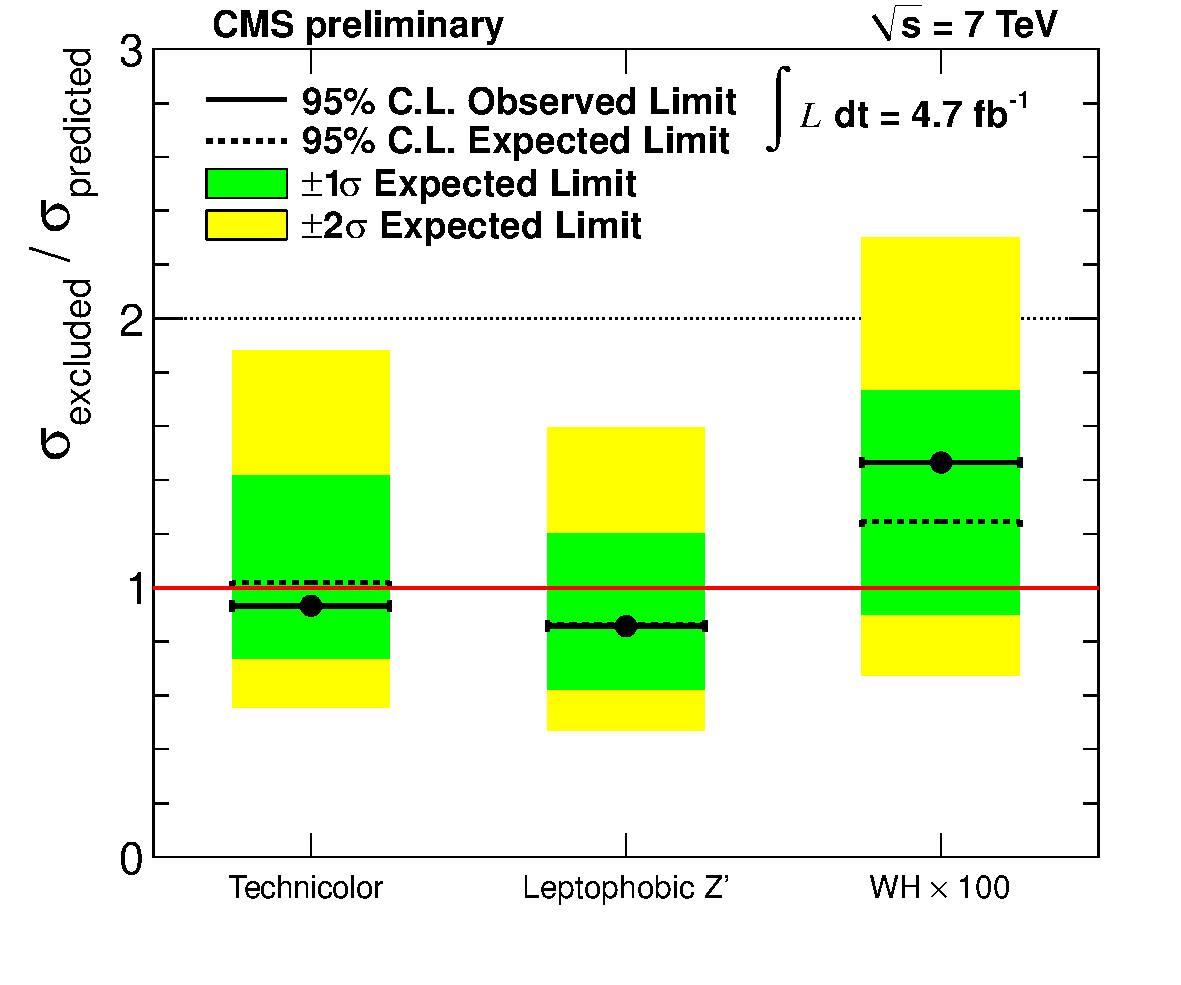
\includegraphics[width=0.45\textwidth]{figs/mjjlimitbars_2+3jet_asymptotic_4p7fb.pdf}
%%}
\subfigure[]{
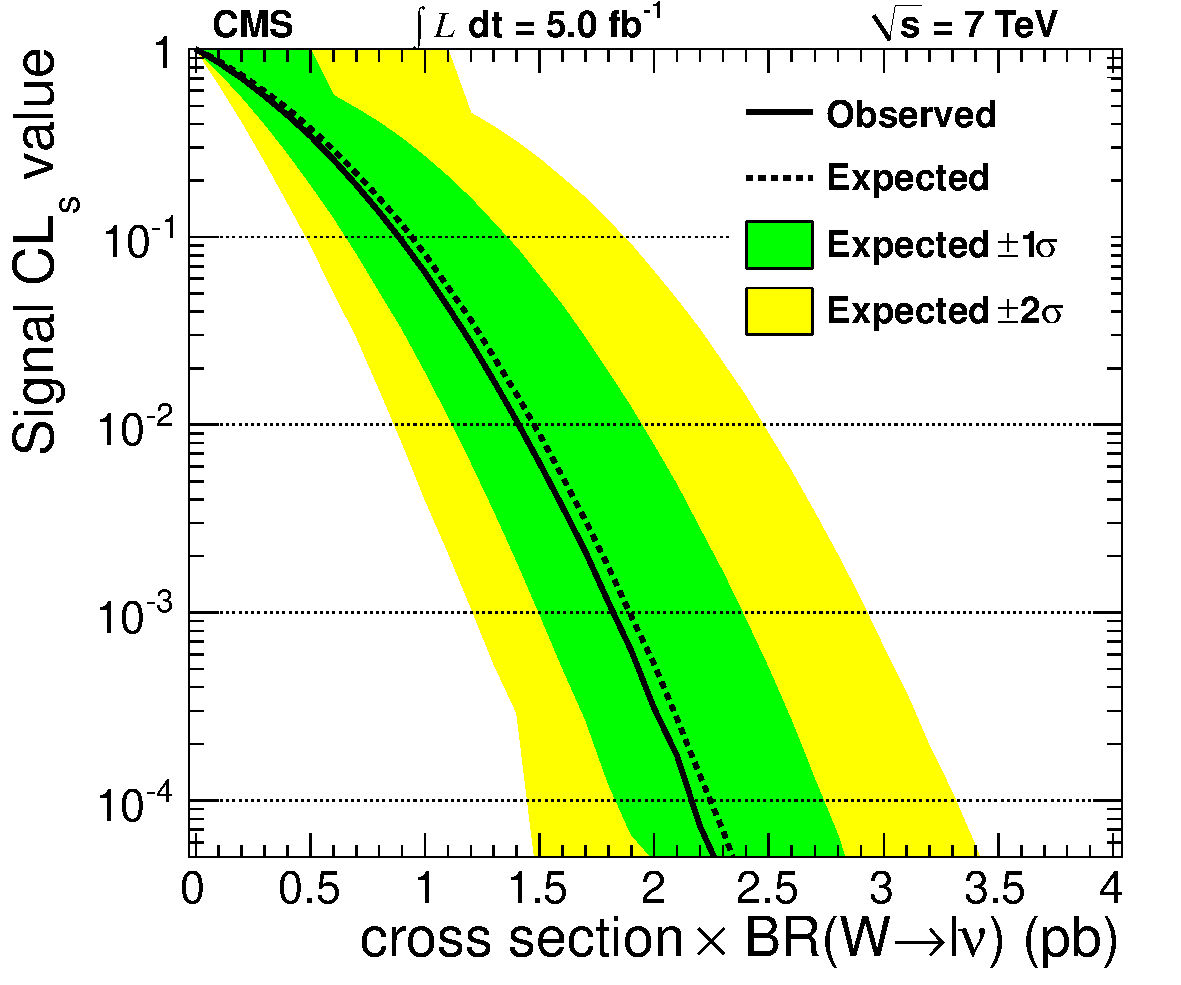
\includegraphics[width=0.45\textwidth]{figs/mjjpvalues.pdf}
}
\subfigure[]{
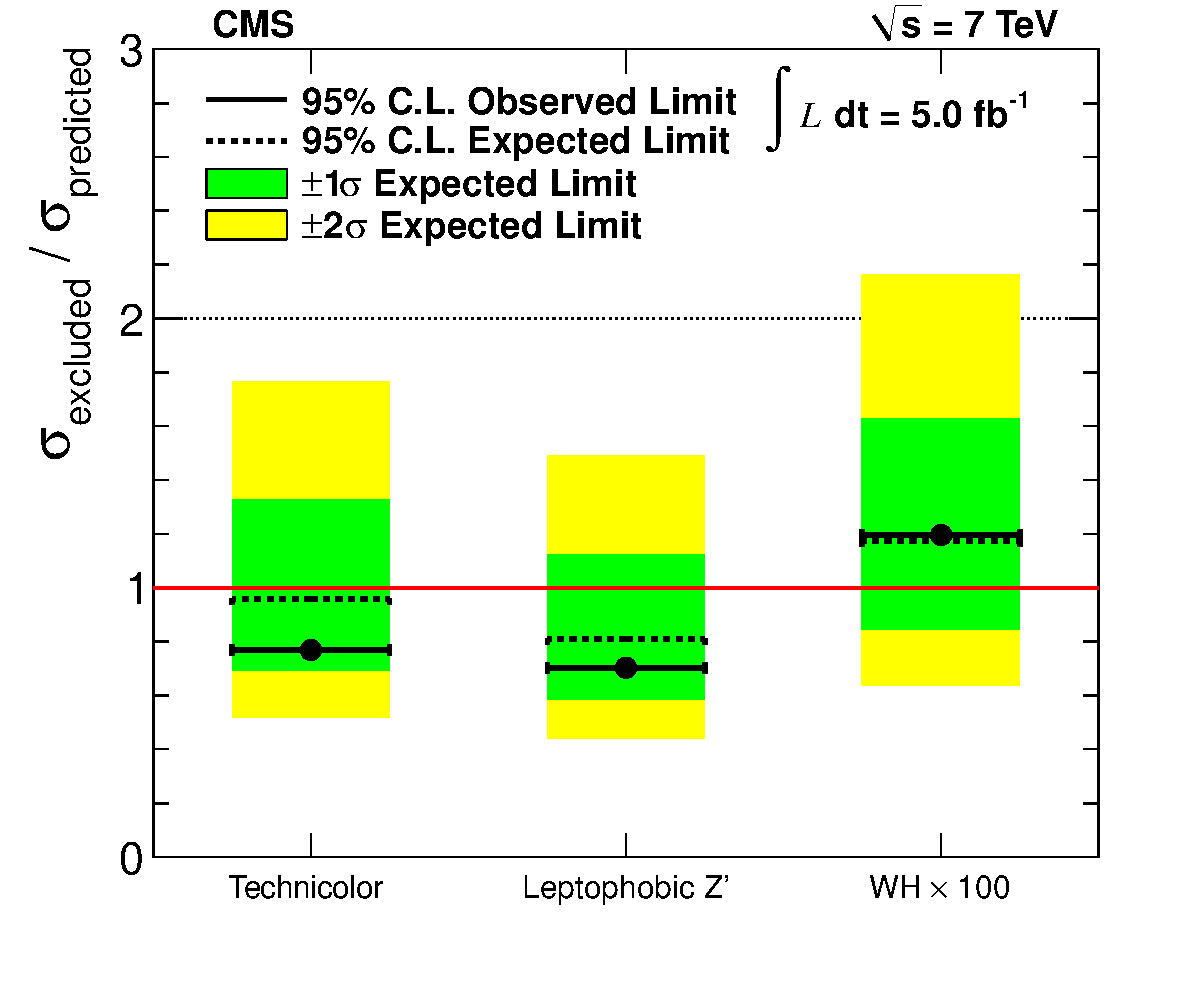
\includegraphics[width=0.45\textwidth]{figs/mjjlimitbars.pdf}
}
\caption{\label{fig:FigLimitsFullData}
(a) The observed and expected values of the CL${}_{\textrm{S}}$ statistic for a
generic Gaussian signal hypothesis with M=150 GeV, width=15 GeV, as a
function of the cross section of the signal times the W$\to\ell\nu$ branching
fraction.
(b) Observed and expected 95\% C.L. upper limits, with 1- and 2-$\sigma$ 
error bands, for technicolor, leptophobic $\Zo^\prime$, and $WH$ signal models. 
}
\end{figure}
%%%%%%%%%%%%%%%%%%%
%%%%%%%%%%%%%%%%%%%%%%%%%%%%%%
%% \subsection{Limits from \texorpdfstring{2.1 fb${}^{-1}$}{2.1/fb} data sample (Runs: 2010+2011A)}
%% The 95\% confidence exclusion limits, based on input shapes from the
%% combined 2+3-jet channels, both with full systematics and with no
%% systematics, are shown in Figure~\ref{fig:mjjlimitbars}. The limits
%% for 2-jet-only and 3-jet-only channels are shown in
%% Figure~\ref{fig:limits2or3}. The figures indicate that, with full
%% systematic errors accounted for, we expect to exclude to better than
%% 95\% confidence a generic Gaussian signal of the strength and
%% invariant mass equivalent to that reported by the CDF collaboration.
%% The observed limits show modest excesses in all cases, 
%% typically within the 2-$\sigma$ band, with the CDF-like signal on the
%% threshold of exclusion. The WH/ZH model had to be artificially scaled
%% by a factor of 150 in order to be compared to the other models.

%% %%%%%%%%%%%%%%%%%%%
%% \begin{figure}[bthp]
%% \subfigure[Nominal 2+3jet shape-based exclusion limit]{
%% 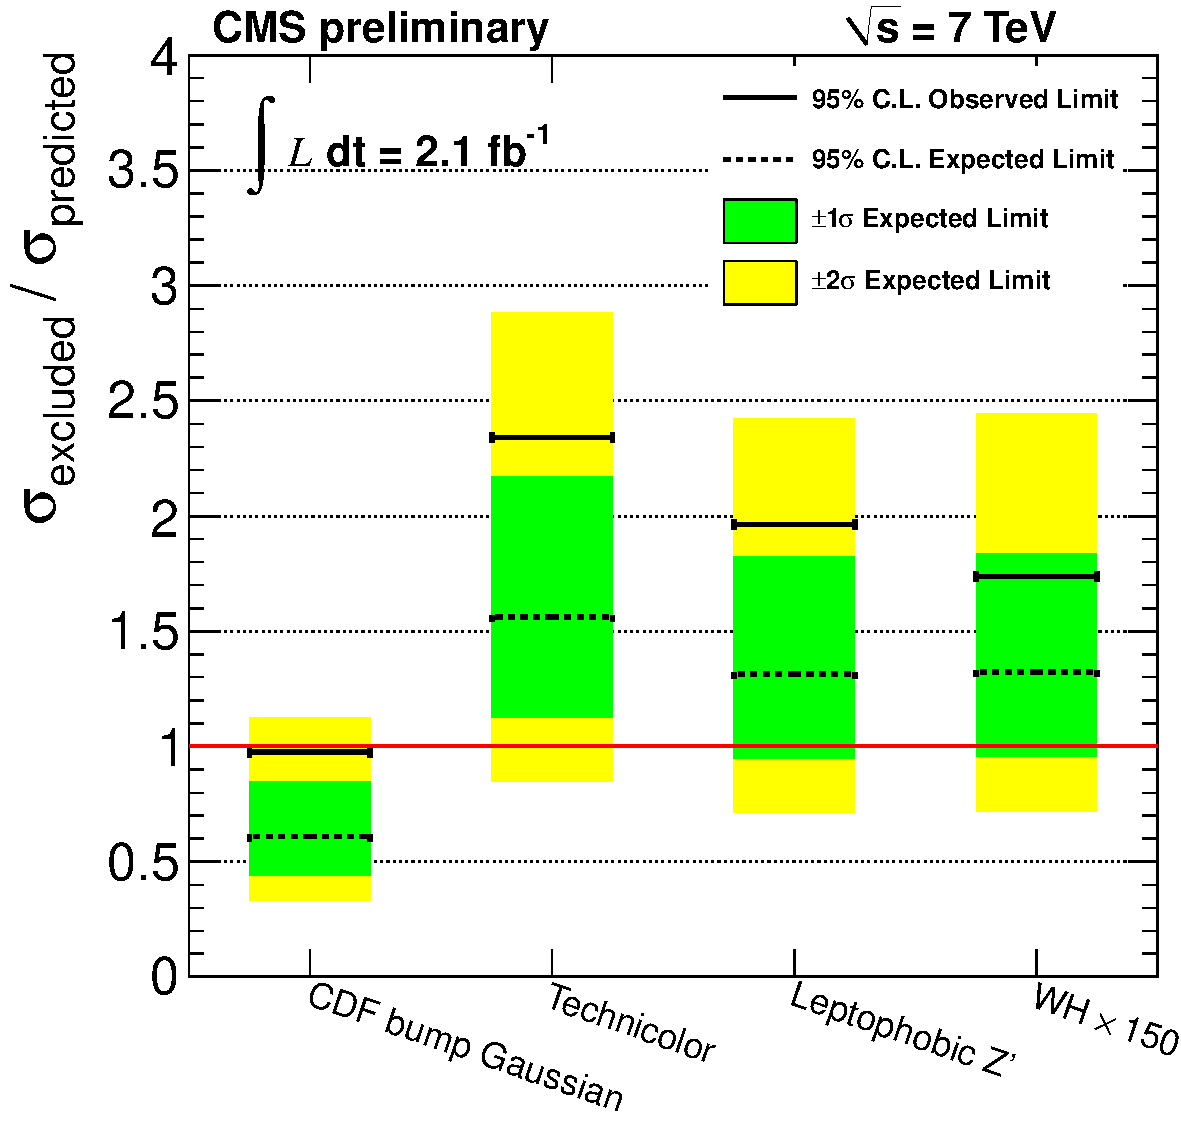
\includegraphics[width=0.45\textwidth]{figs/mjjlimitbars_2+3jet_asymptotic}
%% }
%% \subfigure[Statistics-only limit]{
%% 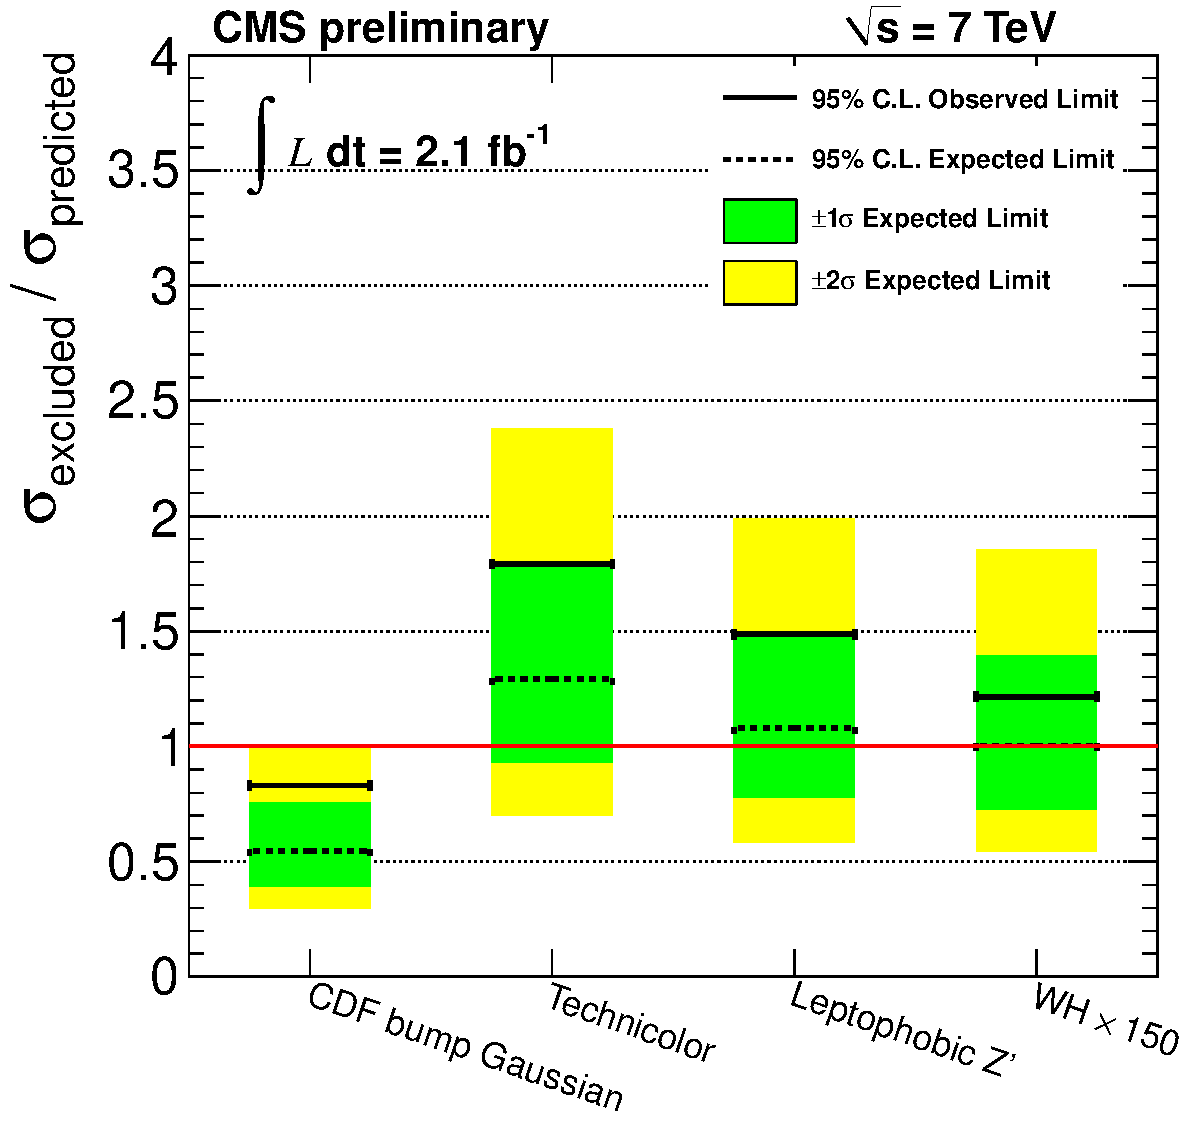
\includegraphics[width=0.45\textwidth]{figs/mjjlimitbars_nosyst.pdf}
%% }
%% \caption{\label{fig:mjjlimitbars}A plot of observed and expected 95\% confidence
%% exclusion limits, with 1- and 2-sigma error bands, for a generic Gaussian
%% signal normalized to the CDF-measured cross-section, as well as for Technicolor,
%% Leptophobic $\Zo^\prime$, and WH signal models. The right plot shows the
%% statistics-only limit while the left plot includes full systematics.}
%% \end{figure}
%% %%%%%%%%%%%%%%%%%%%
%% \begin{figure}[h!]
%% \subfigure[2-jet-only exclusion limit]{
%% 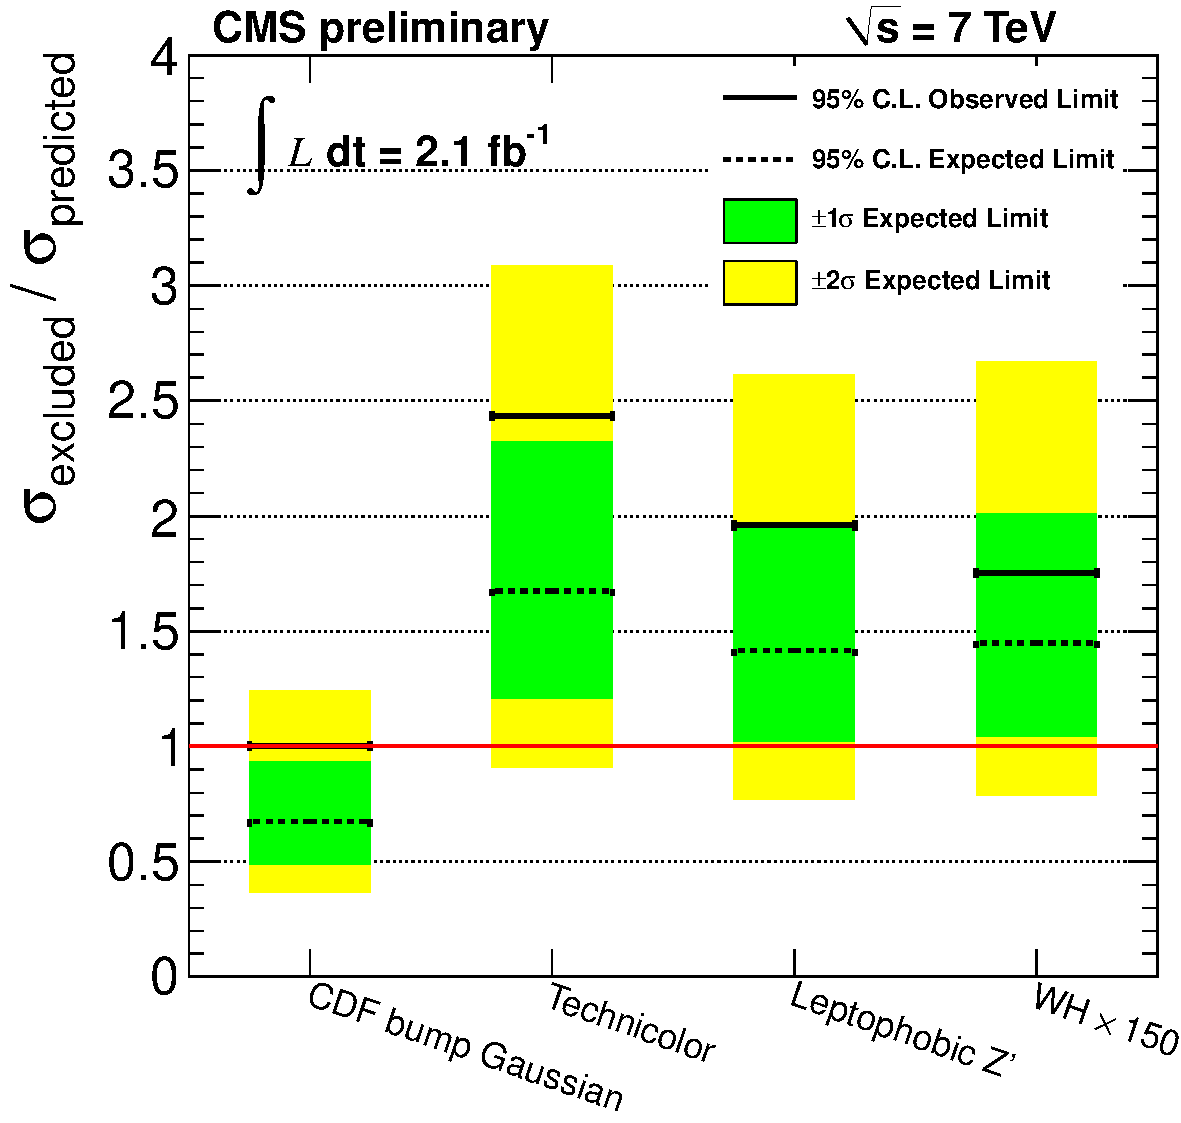
\includegraphics[width=0.45\textwidth]{figs/mjjlimitbars_2jet_asymptotic.pdf}
%% }
%% \subfigure[3-jet-only exclusion limit]{
%% 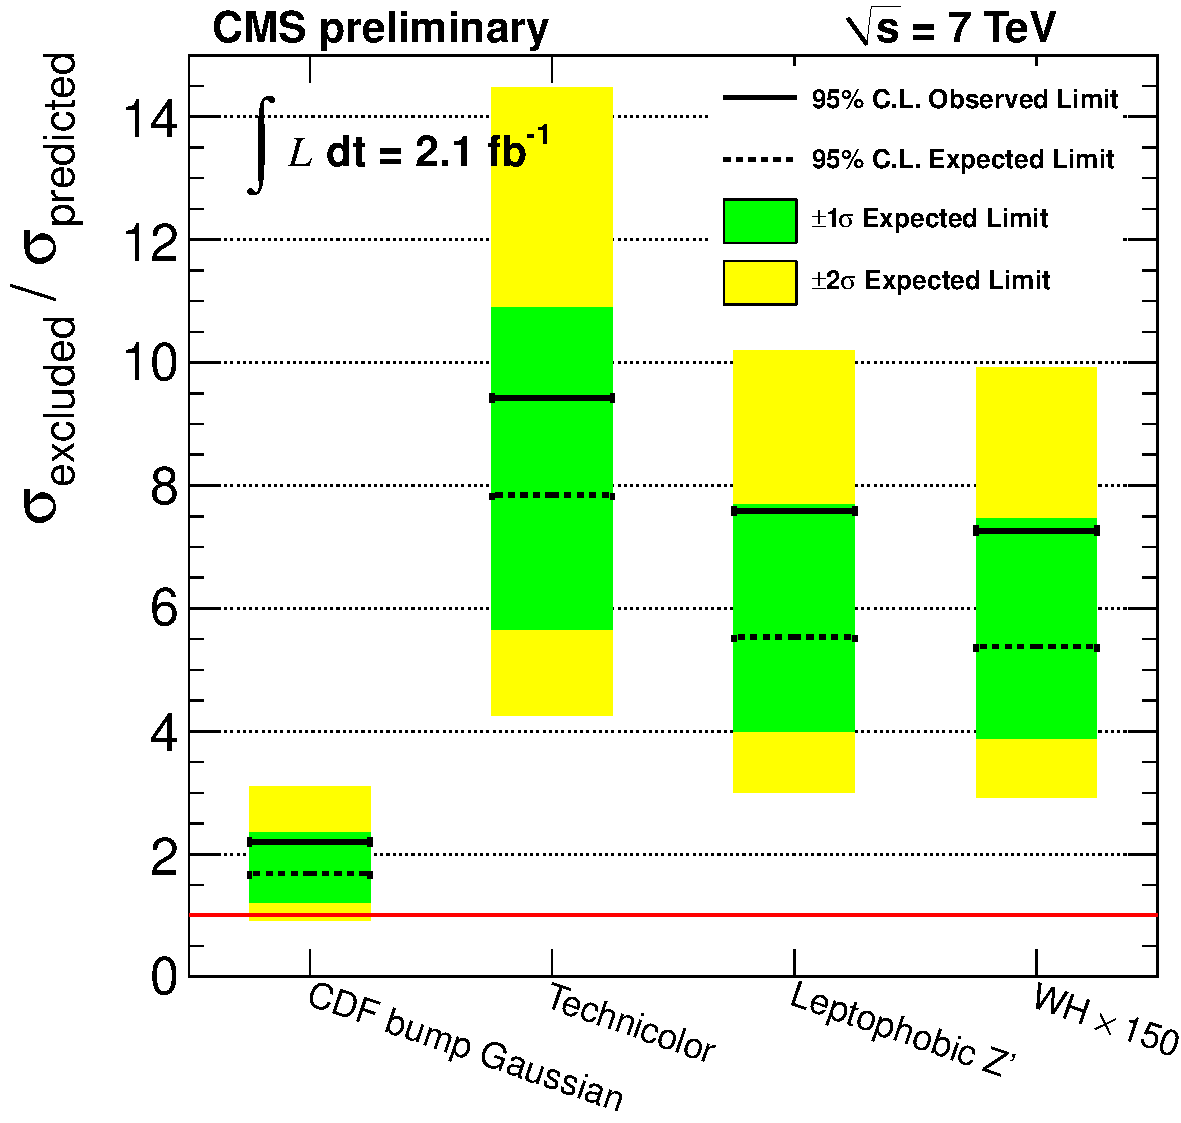
\includegraphics[width=0.45\textwidth]{figs/mjjlimitbars_3jet_asymptotic.pdf}
%% }
%% \caption{\label{fig:limits2or3}Comparison of the upper exclusion
%% limits set on the 2-jet(left) and 3-jet (right) channels separately.}
%% \end{figure}

%% %%%%%%%%%%%%%%%%%%%
%% For a model-independent result, we form a generic Gaussian signal
%% similar to that described above. However, this signal is normalized to
%% a total yield corresponding to the measured luminosity multiplied by a
%% $\sigma\times BR = 1$~pb, with $\epsilon\times\cal{A}$ factors applied
%% that are equal to those measured for the WH signal model. The
%% corresponding shapes from these signal distributions are fed to the
%% limit setter. The limit setter is set to throw 500k pseudo-experiments
%% for each of several fixed values of the ``signal strength'', a
%% unitless scale factor that multiplies the signal normalization. Each
%% pseudo-experiment is drawn from the signal plus background (``s+b'')
%% distribution and yields a p-value of the s+b hypothesis for that
%% experiment.  From a collection of these p-values, the observed, median
%% expected and $\pm$1- or 2- sigma bands for each point are determined
%% and plotted. Since the generic Gaussian model is normalized to 1~pb,
%% this means that a model-independent scan of cross sections in units of
%% picobarns is performed. The results are shown in
%% Fig.~\ref{fig:mjjpvalues}. 
%% %%%%%%%%%%%%%%%%%%%
%% \begin{figure}[htbp]
%% \begin{center}
%% 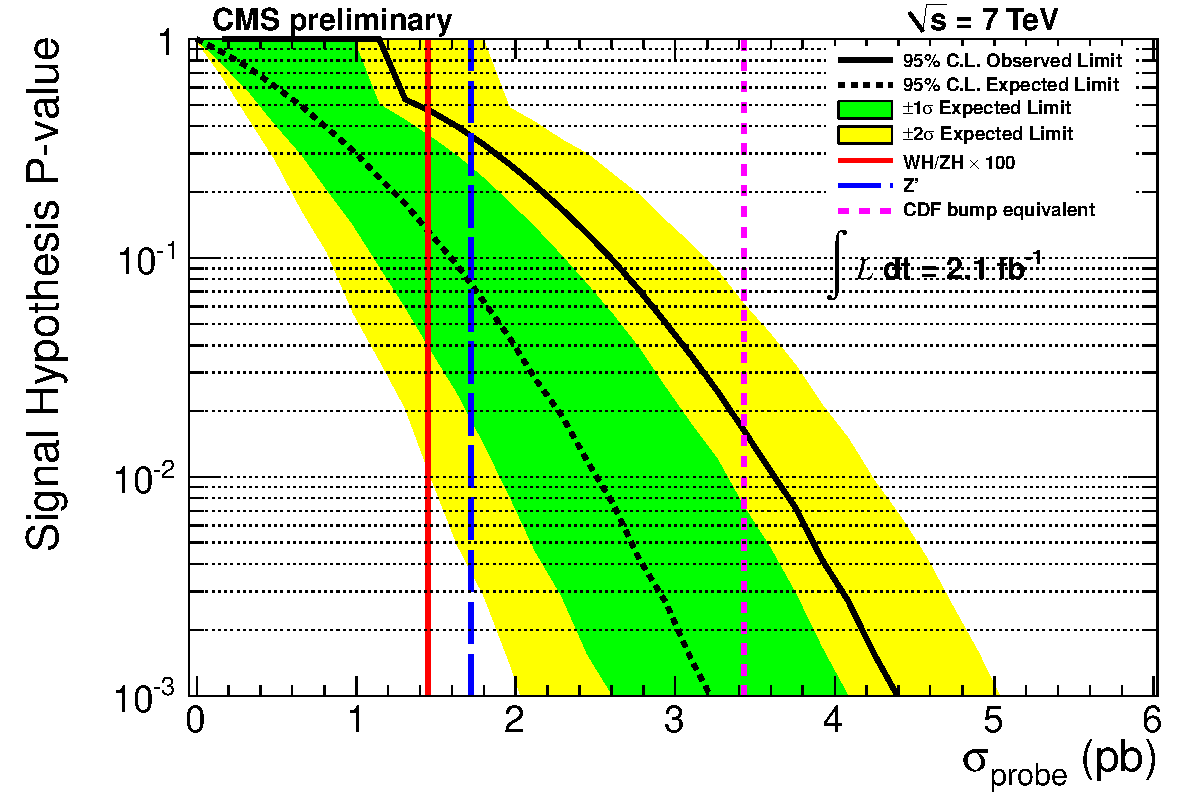
\includegraphics[width=0.8\textwidth]{figs/mjjpvalues_gs2+3jet}
%% \caption{\label{fig:mjjpvalues}A plot of signal p-values (after including 
%% systematic uncertainties) testing the signal+background
%% hypothesis for generic signal models with the given cross-section.}
%% \end{center}
%% \end{figure}
%%%%%%%%%%%%%%%%%%%%%
%% \begin{figure}[bthp]
%% \begin{center}
%% 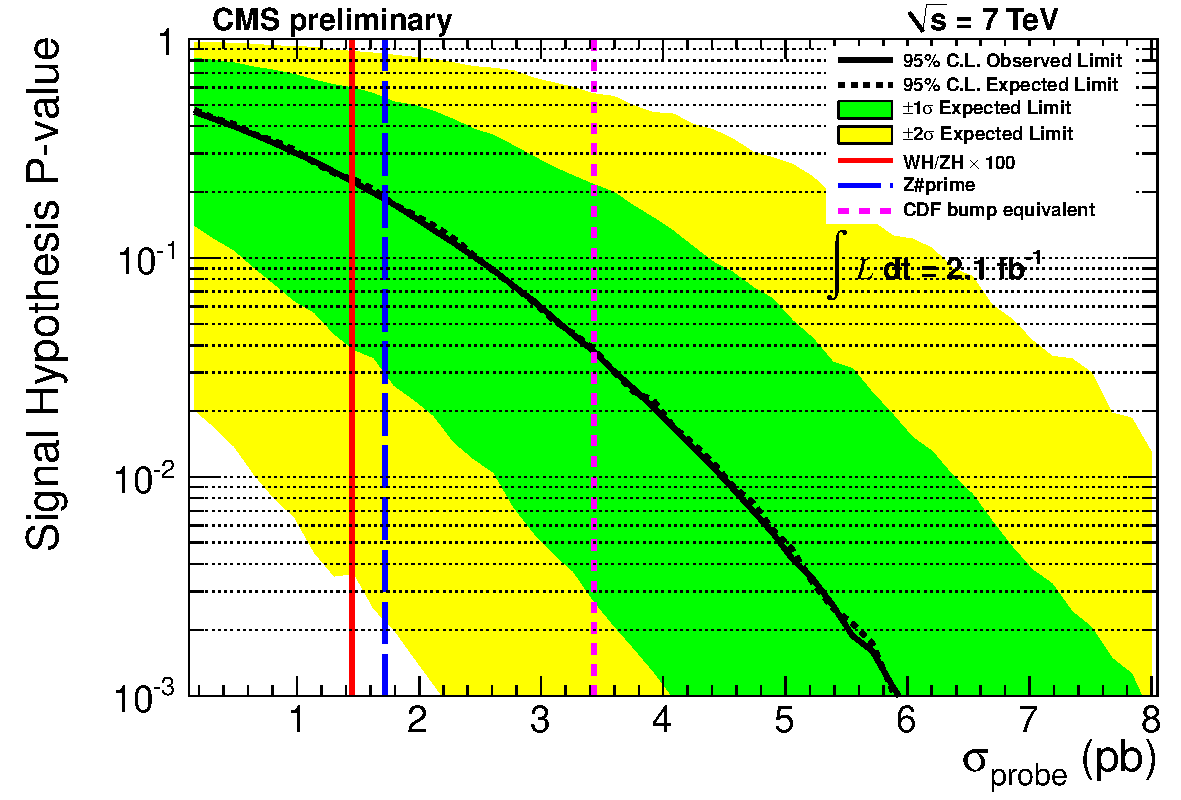
\includegraphics[width=0.8\textwidth]{figs/mjjpvalues_gs2+3jet_nosyst}
%% \caption{\label{fig:mjjpvalnosyst}======== FIXME: Phil will update this plot: it is buggy. =========== The same plot as Fig~\ref{fig:mjjpvalues} of 
%% p-values but using only statistical uncertainties (\textit{i.e.}, no systematic 
%% uncertainties).}
%% \end{center}
%% \end{figure}
%%%%%%%%%%%%%%%%%%%%
%%%%%%%%%%%%%%%%%%%%%
%% \begin{figure}[bthp]
%% \begin{center}
%% \includegraphics[width=0.8\textwidth]{figs/mjjexclusionVsMass_gs2+3jet}
%% \caption{\label{fig:mjjexclusionVsMass}======== FIXME: Phil is working on this plot. =========== The 95\% exclusion limit on the production rate of CDF-size anomaly as a function of dijet mass (in range 130--170 GeV).}
%% \end{center}
%% \end{figure}
%%%%%%%%%%%%%%%%%%%%
